\chapter{Network Layer}\label{C:NetworkLayer}

The first part of this chapter presents the new network system architecture and compares it with previous one.

The following subsections describe each of its main components and present results in order to measure and compare the performance with the old design. The key performance parameters analyzed depending on the architecture component are: simultaneous connections, round-trip time (RTT) and memory allocation.

\section{Architecture}\label{S:Architecture}

The network layer is the lowest level layer on the MAREA stack. This layer it is on charge of provide an optimized, modular and reusable usage of the network capabilities. MAREA network system architecture consist of two main sublayers: encoder and transport.

%width=\linewidth
\begin{figure}[H]\begin{center}
 \centering
  \captionsetup{justification=centering}
  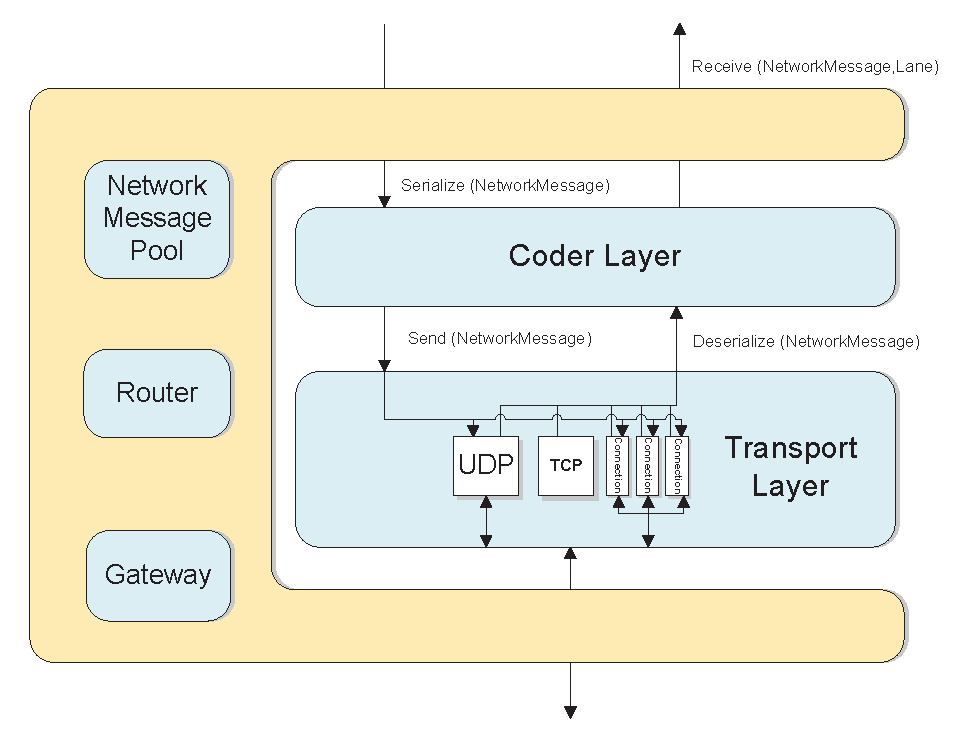
\includegraphics[scale=0.8]{pictures/network/Network}
  \caption{MAREA 2 network layer architecture \label{fig:network-architecture}}
\end{center}\end{figure}

One one hand, the encoder layer is responsible of code MAREA protocol messages into byte sequences. This component also undertakes the inverse operation of decode byte sequences into MAREA protocol messages. 

On the other hand, the transport layer is on charge of send and receive data (byte sequences) from the underlying network through different types of transports (UDP, TCP).

The idea of the proposed design, in order to improve the performance in terms of speed,  is to minimize the amount of time used by the garbage collector to create and destroy object instances.  The architecture component called NetworkMessage pool achieves this improvement using a memory pool mechanism.

The network layer is a highly reconfigurable system that allows the use of different types of encoders and transports. The router is the main component that select this components dynamically. This module it also can be configured by the user of the middleware depending on the scenario.  

The gateway module is on charge of interconnect networks that use different types or protocols and architectures. Its main goal is the translation of the source network protocol to the destination network protocol, and vice versa, in order to allow the communication between them.

In order to provide uniformity and simplicity to the design of each sublayer, the communication between them is done using a common interface. Each of the sublayers send and receive a NetworkMessage entity (figure \ref{fig:network-message}) to the upper and lower layers. This common data structure, which contains all the necessary information used by the encoding and transport layers, is modified as it travels downward or upward the architecture. 

\begin{figure}[H]\begin{center}
 \centering
  \captionsetup{justification=centering}
  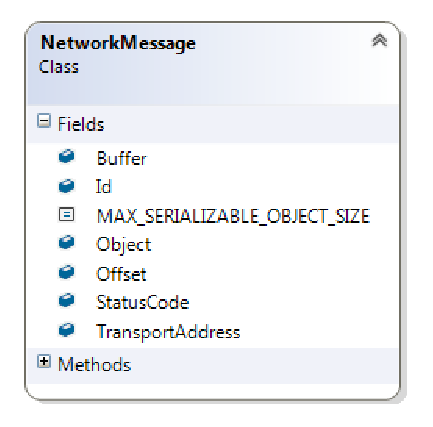
\includegraphics[scale=0.75]{pictures/network/NetworkMessage}
  \caption{NetworkMessage entity \label{fig:network-message}}
\end{center}\end{figure}

One one hand, when encoder sublayer serializes a MAREA message (which is actually stored in the field Object of the NetworkMessage entity), the resulting byte stream is saved in the Buffer field. At the same time, the total length of the serialized data is assigned to the field Offset.

On the other hand, the deserialized incoming MAREA messages are stored in the field Object according to the byte stream and the length of the received data provided by the transport sublayer (this information is contained in the fields Buffer and Offset respectively). 

In relation to the transport layer, when a message is received the fields StatusCode and TransportAddress are set in order to inform the upper layers about the reception status and the source of MAREA message.

\subsection{Comparison with MAREA 1 Network Architecture}\label{SS:Comparison-with-MAREA-1-Network-Architecture}

One of the main differences between the old and new MAREA network designs is the top entry point of the architecture which is called Lane manager. This component is the responsible to control which transports and encoders are used by the middleware at a particular moment. In contrast, the router is the responsible of perform this task in the new architecture.

%width=\linewidth
\begin{figure}[H]\begin{center}
 \centering
  \captionsetup{justification=centering}
  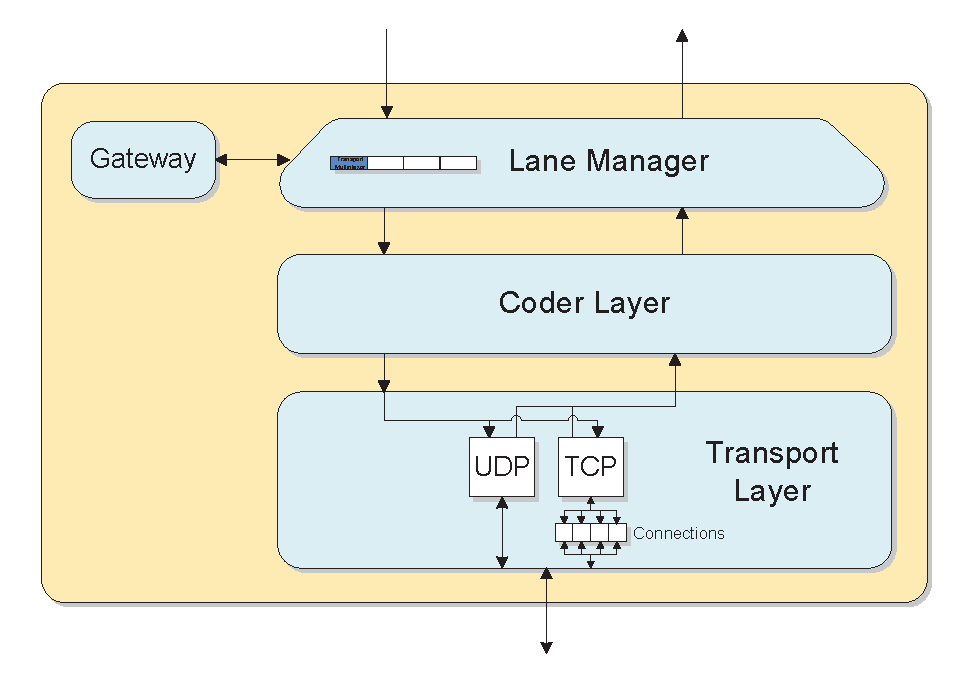
\includegraphics[scale=0.8]{pictures/network/NetworkOld}
  \caption{MAREA 1 network layer architecture \label{fig:network-old-architecture}}
\end{center}\end{figure}

As opposite of the new architecture, network lanes (subsection \ref{SS:Network-Lanes}) are not a set of references to the bindings establish between the different network architecture elements. Instead of this, there are object references (copies) to these elements.

The main idea of taking out the Lane manager in the new architecture is to simplify the design and improve the speed by removing unnecessary repeated searches to the lane, which in normal conditions is always the same. Every time a message is sent in MAREA 1 network architecture, a search has to be done into dictionary in order to get the default lane.

\begin{figure}[H]\begin{center}
 \centering
  \captionsetup{justification=centering}
  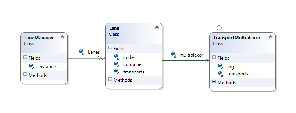
\includegraphics[scale=2]{pictures/network/LaneManager}
  \caption{Lane manager class diagram \label{fig:lane-manager}}
\end{center}\end{figure} 

The new design does not use a dictionary in order to avoid slowdowns in the performance. Instead of this, the network layer use only one output and input lane for the outgoing and incoming data respectively. This lanes are reused while the network continues to work properly. 

The service container, which is the immediate upper layer, is the responsible of keep and provide the hint to the network layer every time. Only if a network change happens, new lanes are demanded to the router. This solution is more complex but reduces the acquisition time of the lanes.

In the transport sublayer, lanes also take profit of its new approach by taking reference directly to the TCP connection which is required in a particular moment instead of searching it in a dictionary.

Another big difference between the two architectures is the sublayer architecture design. For one hand, the MAREA 2 network sublayers (figure \ref{fig:network-architecture}) are uniform. In MAREA 1 the network sublayers (figure \ref{fig:network-old-architecture}) are inconsistent because every single sublayer presents different interfaces in order to communicate with to the upper and lower sublayers. 

For the other hand, in the old architecture every sublayer is dependent of the upper and lower one because it has to keep a reference in order to communicate with them. The new sublayer architecture is more independent and flexible, because the responsibility of manage the bindings between the different sublayers is delegated to the network lanes instead of the sublayers by itself.

Another difference, that has been mentioned before, is the pooling mechanism used in the new architecture which is explained in section \ref{S:Network-Message-Pool}.

\section{Router}\label{S:Router}

MAREA is able to use different encoders and transports in order to to build a modular and configurable network architecture. The router has the ability to select the elements (encoders and transports), of the layered network architecture, at execution time depending on needs and the state of the network. The main aim of this element is to create and manage the network lanes.

\subsection{Network Lanes}\label{SS:Network-Lanes}

A network lane can be defined as a set of references to the bindings establish between the different network architecture elements (encoder and transports) used at a particular moment. Lanes have been implemented as linked lists of delegates or multicast delegates. A delegate is an object that allows the programmer to encapsulate a reference to a method (but is similar to a function pointer in C or C++ but is object-oriented, type-safe, and secure) \cite{cite:delegate}.

The following characteristics of multicast delegates have been taken in account to create network lanes:

\begin{itemize}
\item The invocation list of multicast delegates is called synchronously and orderly.
\item If an exception occurs in a delegate, the remaining delegates of the list are not invoked.
\end{itemize}

According to the figure \ref{fig:network-message} the router use at least two different network lanes to send and receive data.

\begin{table}[H]
\begin{center}
\caption{\nohyphens{Output and input network lanes}}
\label{T:Lanes}
\begin{tabular}{|l|p{7.3cm}|}
\hline
 {\bf Lanes} & {\bf Invocation List} 												\\ \hline \hline
 Output Lane & MareaCoder.Serialize(NetworkMessage m)\newline Transport.Send(NetworkMessage m)\\ \hline
 Input Lane & Coder.Deserialize(NetworkMessage m)\newline Container.Receive(NetworkMessage m)\\ \hline
\end{tabular}
\end{center}
\end{table}

A way to trap link loss or disconnection exceptions it is required in order to notify the upper layers that an error has occurred. There exist two different solutions to this issue:

\begin{itemize}
\item Use the method GetInvocationList to get each individual delegate from the multicast delegate and invoke each delegate within the try block of an exception handler. This solution is very powerful but it has counterparts like the use of system resources and execution time due to the handling of exceptions. 
\item Use a field in the NetworkMessage entity as a status code (figure \ref{fig:network-message}).
\end{itemize}

The second alternative has been implemented in order to accomplish with the objective of improve the performance. 

\section{NetworkMessage Pool}\label{S:Network-Message-Pool}

The non deterministic process of garbage collection is executed .NET virtual machine in order to maintain the memory clean. This process can introduce non deterministic pauses into the execution of a program which are not correlated with the algorithm being processed.

One solution in order to reduce garbage collection interruptions is use a memory pooling mechanism. The main idea of this type of mechanisms is to provide a managed set of functions in order to allocate and deallocate memory. The use of pooling mechanisms keep references to object instances that are beyond destruction, allowing it to be reused when needed. With this technique no objects (NetworkMessage entities) are released to be garbage collected until the middleware is shut down.

The proposed design to implement a memory pool mechanism is to use a FIFO queuing discipline for NetworkMessage entities. In this common queue disciple, the elements are added to the tail are removed from the head using a pair of object references to the tail and the queue.

The final purpose of the NetworkMessage pool is to reduce the amount of work that has to be done by the garbage collector in order to minimize the time used by its own execution. 

\subsection{Results}\label{SS:Network-Message-Pool-Results}

A memory allocation profiling test has been executed in order to evaluate the behavior of the NetworkMessage pool. The figure \ref{fig:pool-memory-allocation} presents the total bytes allocated by MAREA 1 and the MAREA 1 network backport (section \ref{S:MAREA-1-Network-Backport}) during a echo request/response test with two MAREA instances. Each instance runs a different service which sends or responds to the messsage. This results correspond to the total bytes allocated by the sender.

The test has been executed 100000 times to send variables (UDP) and events (TCP) primitives with a total payload of 1000 bytes and frequency of 100 Hz. MAREA 1 network backport has been tested in two different modes: reusing network lanes and creating every time on demand. 

\begin{figure}[H]\begin{center}
 \centering
  \captionsetup{justification=centering}
  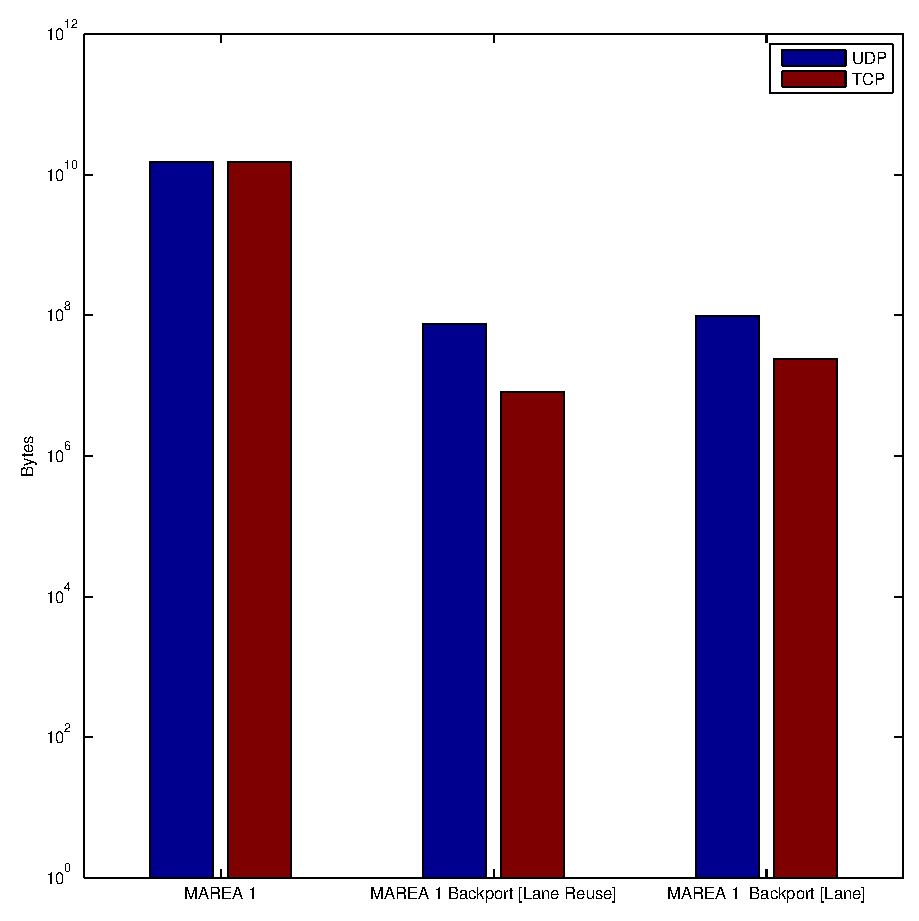
\includegraphics[scale=0.6]{pictures/network/MemoryAllocationBackport}
  \caption{Total bytes allocated in MAREA 1 and MAREA 1 network backport (1000 Bytes, 10000 packets, 100 Hz) \label{fig:pool-memory-allocation}}
\end{center}\end{figure}

\section{Encoding Layer}\label{S:Encoding-Layer}
The encoding layer is on charge of serializing and deserializing MAREA messages. This layer provides an abstraction layer such all logic above contained in the upper-layers does not need to know the particulars about how messages are serialize and deserialized.

Serialization is the act of taking an in-memory object or object graph (set of objects that reference each other) and flattening it into a stream of bytes \cite{cite:serialization}. The reverse operation is deserialization which takes a data stream and regenerates into an in-memory object or object graph.

\subsection{Previous Work}\label{SS:Encoding-Layer-Previous-Work}
The initial version of MAREA has been implemented with the idea of providing several encoding layer implementations (XML serialization, binary serialization and MAREA coder) in order to allow adaptability and interoperability between the devices and the network. The first two implementations of the encoding layer use .NET Framework serialization mechanisms such as binary serialization through BinaryFormatter class, and human-readable XML serialization through XMLSerializer class.

The BinaryFormatter is easy to use and automatic, but it is not such flexible as XMLSerializer. For the other hand XMLSerializer is slower and less powerful because it is not able to restore shared object references.  Furthermore, XML serialization does not convert private fields, indexers, methods, or read-only properties (except read-only collections). In order to do this, is mandatory to use the BinaryFormatter class.

\begin{table}[H]
\begin{center}
\caption{\nohyphens{Serialization engine comparison between .NET BinaryFormatter and XMLSerializer}}
\label{T:NetBinaryXML}
\begin{tabular}{|l|c|c|}
\hline
{\bf Feature} & {\bf BinaryFormatter} & {\bf XMLSerializer}          \\ \hline \hline
Level of automation                            & *****   & ****      \\ \hline
Type coupling                                  & Tight   & Loose     \\ \hline
Version Tolerance                              & ***    & *****      \\ \hline
Can serialize nonpublic fields                 & Yes   & No           \\ \hline
Preserves the object reference        		   & Yes   & No           \\ \hline
Suitability for interoperable messaging        & **    & ***         \\ \hline
Flexibility in reading/writing XML files       & -     & ****        \\ \hline
Compact output                                 & ****  & **           \\ \hline
Performance                                    & ****  & * To ***       \\ \hline
\end{tabular}
\end{center}
\end{table}

One of the main drawbacks of these two mechanisms is the performance overhead. Serializing a message with BinaryFormatter is expensive because of the metadata present. This is more noticeable in XMLSerializer because the overhead introduced by the XML tags is bigger. 

Another disadvantage of these two mechanisms is the interoperability between the different virtual machine representations of .NET Frameworks. For instance, XML serialization is not available on the Micro Framework and binary serialization works different in .NET Framework and .NET Compact Framework.

The last implementation of the encoding layer, which is called MAREA coder, has been designed in order to solve these two drawbacks controlling the serialization and deserialization of the different types. This technique, allows the programmer to have more control over the serialization and deserialization processes and ensures serialization compatibility.

The first implementation of this encoder was made using introspection to serialize and deserialize each message dynamically. The results of this first approach were not satisfactory in terms of speed because introspection it is a slow process. Custom serialization solves this issue by using specific methods or routines to serialize and deserialize specific MAREA messages.

MAREA coder has better performance in terms of speed and serialized data size than .NET BinaryFormatter and XMLSerializer implementations. MAREA coder is not dependent of the .NET Framework, so the interoperability between different virtual representations of the .NET Frameworks is not a problem like in .NET BinaryFormatter and XMLSerializer implementations.

\subsection{Drawbacks}\label{SS:Encoding-Layer-Drawbacks}
MAREA coder has some drawbacks inherited from custom serialization like complexity, especially in those cases like tree of objects or object graphs that might contain cycles. In these cases the code could be really hard to study. 

Another point that has to be taken in account of this approach is development speed. Custom serialization does take time for testing, developing and maintenance. For instance, if some messages are added or modified in the protocol layer, the corresponding methods to serialize and deserialize these messages must be added or modified too in order the encoder layer continues to work properly.

MAREA coder has been designed with two serialize and deserialize entry point methods that implement a large switch statement to get the type of object that has to be serialized/deserialized. A large switch statement means the method is large, hard to read and can generate very high complexity metrics.

\subsection{Improvements}\label{SS:Encoding-Layer-Improvements}
The following subsection presents an alternative design for the encoding layer in order to solve the drawbacks of MAREA coder.  

The new proposed design is based on an automatic tool called MAREAGen. This tool generates classes automatically with methods to serialize and deserialize MAREA entities marked as serializable. This eliminates the need for developers to implement serializing and deserializing code and guarantees run-time type safety.

Serialize and deserialize methods have been implemented as static because they have no instance. This type of methods is slightly faster than instance methods because are called with type name instead of an instance identifier. Serialize and deserialize methods also include inlining through the method implementation option agreessive inlining (Listing \ref{lst:SlowData}). This option allows compiler to eliminate the cost of method calls if it is possible. 

\begin{lstlisting}[caption={Class to serialize/deserialize MAREA SlowData messages },label={lst:SlowData}]
public class MG_SlowData
{
  /**
  * This static constructor is called by MAREA in order to load 
  * and register the identifier and specific methods to serialize
  * and deserialize this type.
  **/
  static MG_SlowData()
  {
    M2CoderTables.GetInstance().AddClass(typeof(Marea.SlowData), 50,
    MG_SlowData.Decode, MG_SlowData.Encode);		
  }

  public static readonly ulong MAREAGEN_FINGERPRINT= 11653293;
  
  /**
  * This method serializes all the different objects contained
  * inside a SlowData message into the given byte array.
  **/
  [MethodImpl(MethodImplOptions.AggressiveInlining)]
  public static void Encode(object theSlowData, byte[] buffer, ref int offset)
  {
    //Serialize fields...
  }

  /**
  * This method deserializes all the different objects of  a
  * SlowData message from the given byte array. This method also
  * returns the whole SlowData object 
  **/
  [MethodImpl(MethodImplOptions.AggressiveInlining)]
  public static object Decode(byte[] buffer, ref int offset)
  {
    SlowData slowdata = new SlowData();
    //Deserialize fields...
    return slowdata;
  }
}
\end{lstlisting}

MAREAGen provides fingerprints in each of every generated class, derived from the type definition, in order to provide an unequivocal and fast way to detect code that had not been recompiled. 

At the end of every execution, MAREAGen generates a XML and a DLL file which contains a list of the generated types with its unique byte code identifier and the generated classes to serialize and deserialize MAREA serializable classes respectively.

The proposed solution to solve the complexity issues is to include a hash table and a array of delegates for serialization and deserialization methods. Each of these collections also stores a reference to the byte code identifier provided by MAREAGen: the key values in case of the hash table and the index in case of the array)

One of the things that has to be accomplished in order to store the delegates into a dictionary is that all of the different serialize and deserialize methods must have a compatible signature (encode and decode methods from Listing \ref{lst:SlowData}).

With this approach, the complexity of having large methods with a lot of switch statements is reduced by moving each of the code sections, for every type of MAREA message, to a specific serialize and deserialize methods. 

Furthermore, the speed performance should be improved using the dictionary with the byte code identifiers, because with this solution long switch statements are avoided. The proposed approach is also more scalable: if the number of MAREA messages grows the serialization time should maintain constant, because it only depends on the time to access time to the delegates contained in the dictionary.

The table \ref{T:Messages-Id} presents the proposed byte code identifier distribution according to the different types used by MAREA Coder. MAREA protocol message identifiers are assigned at the beginning in order to reuse them in the service container. Similar to the encode layer, the service container has an array of delegates used to process each MAREA protocol message according to its identifier. In this case the position of the delegates inside the array correspond to the MAREA protocol message byte code identifier.

\begin{table}[H]
\begin{center}
\caption{\nohyphens{MAREAGen identifier distribution}}
\label{T:Messages-Id}
\begin{tabular}{|l|p{7.3cm}|}
\hline
 {\bf Id} & {\bf Type} 												\\ \hline \hline
 From 0 to 63 & MAREA protocol messages\\ \hline
 64 & Null\\ \hline
 From 65 to 126 & MAREA Coder basic types \\ \hline
 127 & Not null\\ \hline
 From 128 to 255 & MAREA Coder types created by MAREAGen\\ \hline
\end{tabular}
\end{center}
\end{table}

Once MAREA is started the DLL file generated from MAREAGen tool is used by MAREA coder in order to add the type code and delegates of the generated classes in the dictionary. This task is performed automatically, running the class constructor methods of classes that have been previously generated by MAREAGen.

Marea coder serialize and deserialize specific methods have also been modified in order to reduce the data size. For instance, the size of serialized System.Double is now reduced from 11 Bytes to 5 Bytes(1 of this 5 bytes is Marea  to encode the number 19 that indicates that the payload is a double).

Another new feature of this implementation is the support for some of the most commonly used  .NET collection types like lists, dictionaries and hash tables. 

The following bugs have also been resolved according to the results obtained in the implemented unit testing with NUnit tool:

\begin{itemize}
\item Compatibility with UTF8 character encoding.
\item Overflow exceptions for high values (double.MaxValue) in double types.
\item Support for run-time/dynamic Enum types.
\item Full support of polymorphic capabilities: Inheritance and control of null objects in object trees.
\end{itemize}
	
\subsection{Results}\label{SS:Encoding-Layer-Results}

The figure \ref{fig:coder-latencies} presents the total serialization and deserialization time for some specific types for the previous and the new implementation of MAREA coder. The most representative type is the specific MAREA message SlowData. This message is used by MAREA to transmit the data of the different MAREA primitives(variables, events, remote invocation, file-based data transfer). This time is 223.49 and 19.64 \textmu s for the old and new implementation respectively. Notice that the y axis in the figure is a logarithmic scale.

\begin{figure}[H]\begin{center}
 \centering
  \captionsetup{justification=centering}
  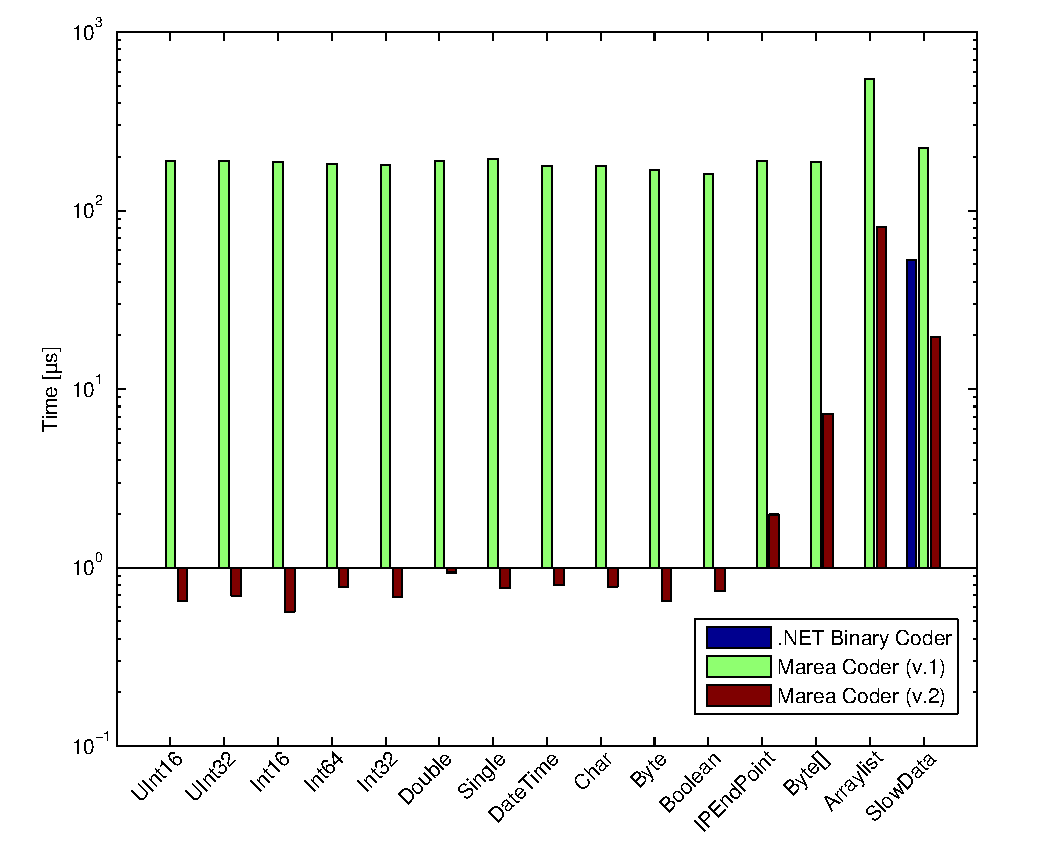
\includegraphics[scale=0.6]{pictures/network/LatencyCoder}
  \caption{Encoder layer implementations: Total serialization and deserialization time\label{fig:coder-latencies}}
\end{center}\end{figure}

The figure \ref{fig:coder-latencies-new-types} presents the total serialization and deserialization time for the new supported types in MAREA coder. This latencies are also compared with the .NET BinaryFormatter coder implementation. 

\begin{figure}[H]\begin{center}
 \centering
  \captionsetup{justification=centering}
  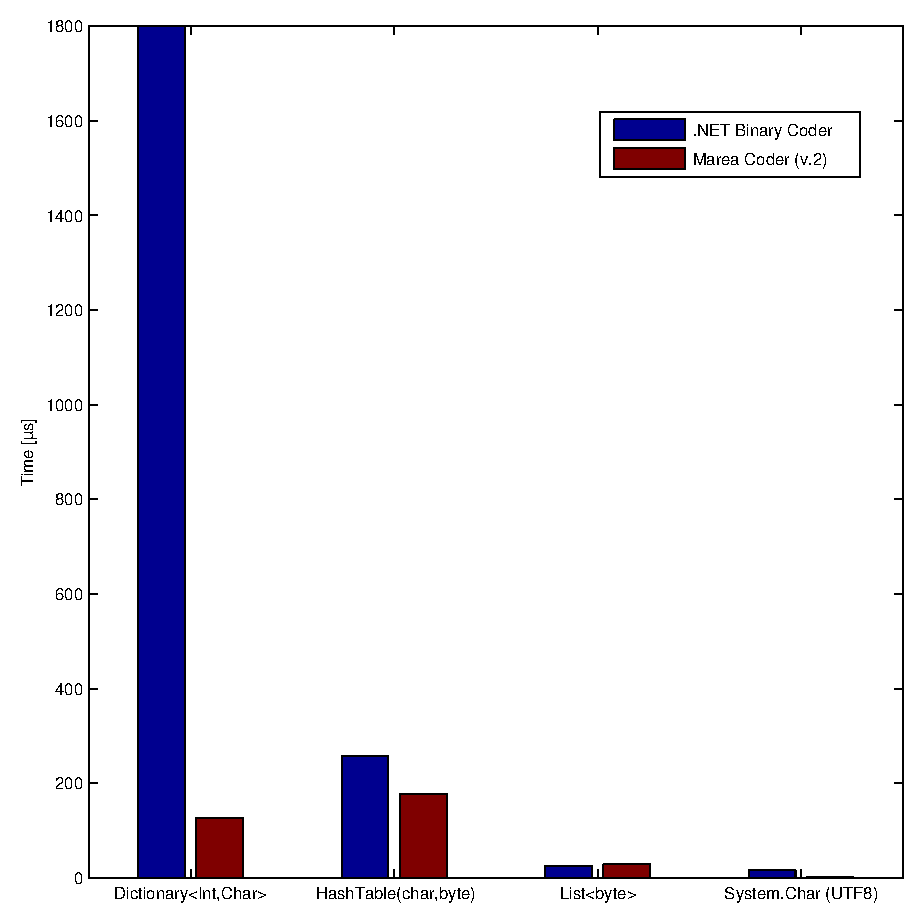
\includegraphics[scale=0.6]{pictures/network/LatencyCoderNewTypes}
  \caption{Encoder layer implementations: Total serialization and deserialization time for new supported types \label{fig:coder-latencies-new-types}}
\end{center}\end{figure}

\section{Transport Layer}\label{S:Transports}

The transport layer provides communication facilities to send and receive data (byte sequences) from the network. This layer provides transfer of data with a certain degree of transparency supporting the two most common transport protocols: TCP and UDP.

TCP transport guarantees reliable end-to-end connection oriented communications. This type of connections require a handshake mechanism in order to negotiate the terms of the connection. The exchange of segments related with this mechanism can adversely affect the performance. 

This problem can be resolved by reusing the established connections instead of opening new TCP connections. The use of persistent connections results in less network traffic, use less time in order to establish new connections and allows the TCP protocol to work more efficiently.

Each MAREA protocol message is sent by TCP transport adding previously a magic number to the corresponding byte sequence representation of itself. This magic number consists in a  synchronization header of 3 bytes followed by an integer (4 bytes) to specify the payload length. The first 3 bytes are use to indicate that the data is synchronized. If this first 3 bytes do not correspond to the expected ones, the transport layer detects that an error condition has happened.

UDP transport provides unreliable (best-effort) datagram comunications. In this type of transport, as the opposite of TCP transport, one stream is opened and closed for the dispatching of each message.

\subsection{Drawbacks}\label{SS:Transports-Drawbacks}

MAREA old transport layer model use the .NET synchronous socket API in order to implement transports. The blocking mode of it set of calls require different threads to accept connections and perform socket I/O operations. 

The use of one thread for each individual connection is non-scalable, especially in Windows systems. The management of a large number of threads is highly inefficient due to the  ineffectiveness of the scheduler to determine which thread should be receiving the processor time. 

The memory overhead is also a handicap. For instance, in Windows the default memory overhead is 1 MB for both native and Common Language Runtime threads.

\subsection{Improvements}\label{SS:Transports-Improvements}

The scalability performance issue can be solved by using asynchronous sockets. Asynchronous I/O operations alleviate the need to create and manage threads \cite{cite:performance-sockets}. This type of sockets use threads internally at the OS Level, which is much faster.

Asynchronous sockets implement specific methods that use  the AsyncCallback class to call completion methods to the following operations: send, receive, connect, accept. Callbacks allow the application to continue processing other events while network operations are been executed.

Two new TCP and UDP asynchronous transport modes have been added in transport layer in order to improve the scalability and the performance.

\subsection{Results}\label{SS:Transports-Results}

Synchronous and asynchronous UDP transports have been compared using a round-trip isolated test. The figure \ref{fig:coder-udp-transports} presents the mean round-trip times during a echo request/response test with simultaneous transports. The mean round-trip time has been calculated according to the average value of the round-trip time of each connection.
 
\begin{figure}[H]\begin{center}
 \centering
  \captionsetup{justification=centering}
  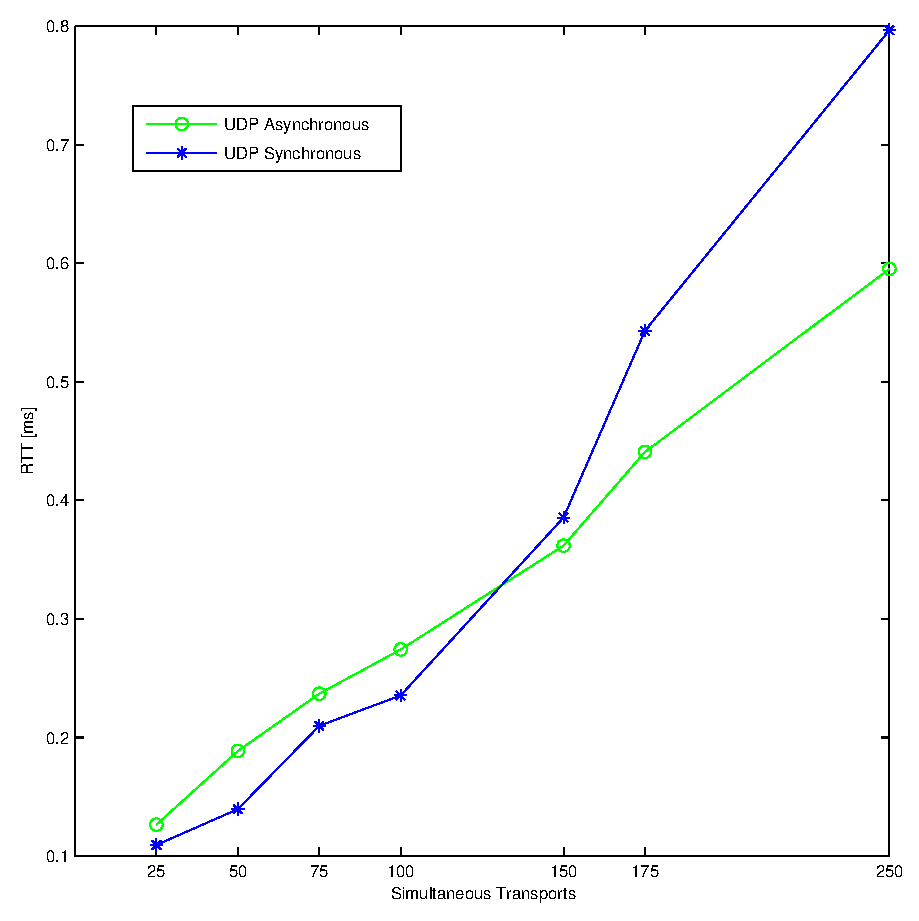
\includegraphics[scale=0.5]{pictures/network/UDPTransports}
  \caption{Mean round-trip times for the echo test using isolated synchronous and synchronous UDP transports (1000 Bytes, 5000 times, 100 Hz) \label{fig:coder-udp-transports}}
\end{center}\end{figure}

According to the results, the round-trip time tends to grow exponentially with the number of simultaneous connections. The round-trip becomes lower in asynchronous mode, in comparison to synchronous mode, from around 150 simultaneous transports. 

\section{MAREA 1 Network Backport}\label{S:MAREA-1-Network-Backport}

The whole new MAREA 2 network architecture has been backported to MAREA 1 in order to ensure its proper functioning. Backporting is the action of taking a certain software modification (patch) and applying it to an older version of the software than it was initially created for \cite{cite:backporting}. This software backport also provides a fair and realistic  way to compare the performance between the old and new network architecture.

\subsection{Results}\label{SS:Backport-Results}

MAREA 1 and MAREA 1 network backport have been compared using a round-trip test. The figure \ref{fig:RRT-backport-UDP} presents the round trip time distribution during a echo request/response test with two MAREA instances. Each instance runs a different service which sends or responds to the messsage. 

The test has been executed 100000 times to send variables (UDP) with a total payload of 1000 bytes and frequency of 100 Hz. The mean round-trip time is 0.2399 and 0.433 ms for MAREA 1 network backport and MAREA 1. The standard deviation is 0.1756 and 0.3813 ms respectively.

\begin{figure}[H]\begin{center}
 \centering
  \captionsetup{justification=centering}
  \includegraphics[scale=0.8]{pictures/network/RTTBackportUDP}
  \caption{Round-trip time distribution for the echo test of MAREA 1 and MAREA 1 network backport using variable primitives (1000 Bytes, 10000 packets, 100 Hz) \label{fig:RRT-backport-UDP}}
\end{center}\end{figure}

The same test has been done using events (TCP). The mean round-trip time is 0.3501 and 0.6564 ms for MAREA 1 network backport and MAREA 1.The standard deviation is 0.2206 and 0.4061 ms respectively.




